\documentclass[spanish]{article}

\usepackage{mystyle}
\usepackage{myvars}
\usepackage{mylinearprogramming}



%-----------------------------

\begin{document}

	\maketitle % Insert title

	\thispagestyle{fancy} % All pages have headers and footers


%-----------------------------
%	ABSTRACT
%-----------------------------

	\begin{abstract}
		\noindent [TODO ]
	\end{abstract}

%-----------------------------
%	TEXT
%-----------------------------

	\section{Introducción}

		\paragraph{}
		[TODO ]

	\setcounter{section}{5}

	\section{Set-Covering Problem}
	\label{sec:e-6}

		\paragraph{}
		[TODO ]

		\begin{eqfloat}
			\begin{equation}
				\begin{array}{ll@{}ll}
					\text{Minimizar}	& \displaystyle\sum\limits_{j=1}^{n} c_{j}	&	x_{j} &\\
					\text{sujeto a}		& \displaystyle\sum\limits_{j = 1}^n a_{ij}	&	x_{j} \geq 1,  &i=1 ,..., m\\
														&                                           &	x_{j} \in \{0,1\}, &j=1 ,..., n
				\end{array}
			\end{equation}
			\caption{Formulación de \emph{Set-Covering Problem}.}
			\label{eq:set_covering}
		\end{eqfloat}


		\subsection{Ejercicio Nueva York}
		\label{sec:e-6.1}

			\paragraph{}
			[TODO ]


			\begin{figure}[h]
				\begin{center}
					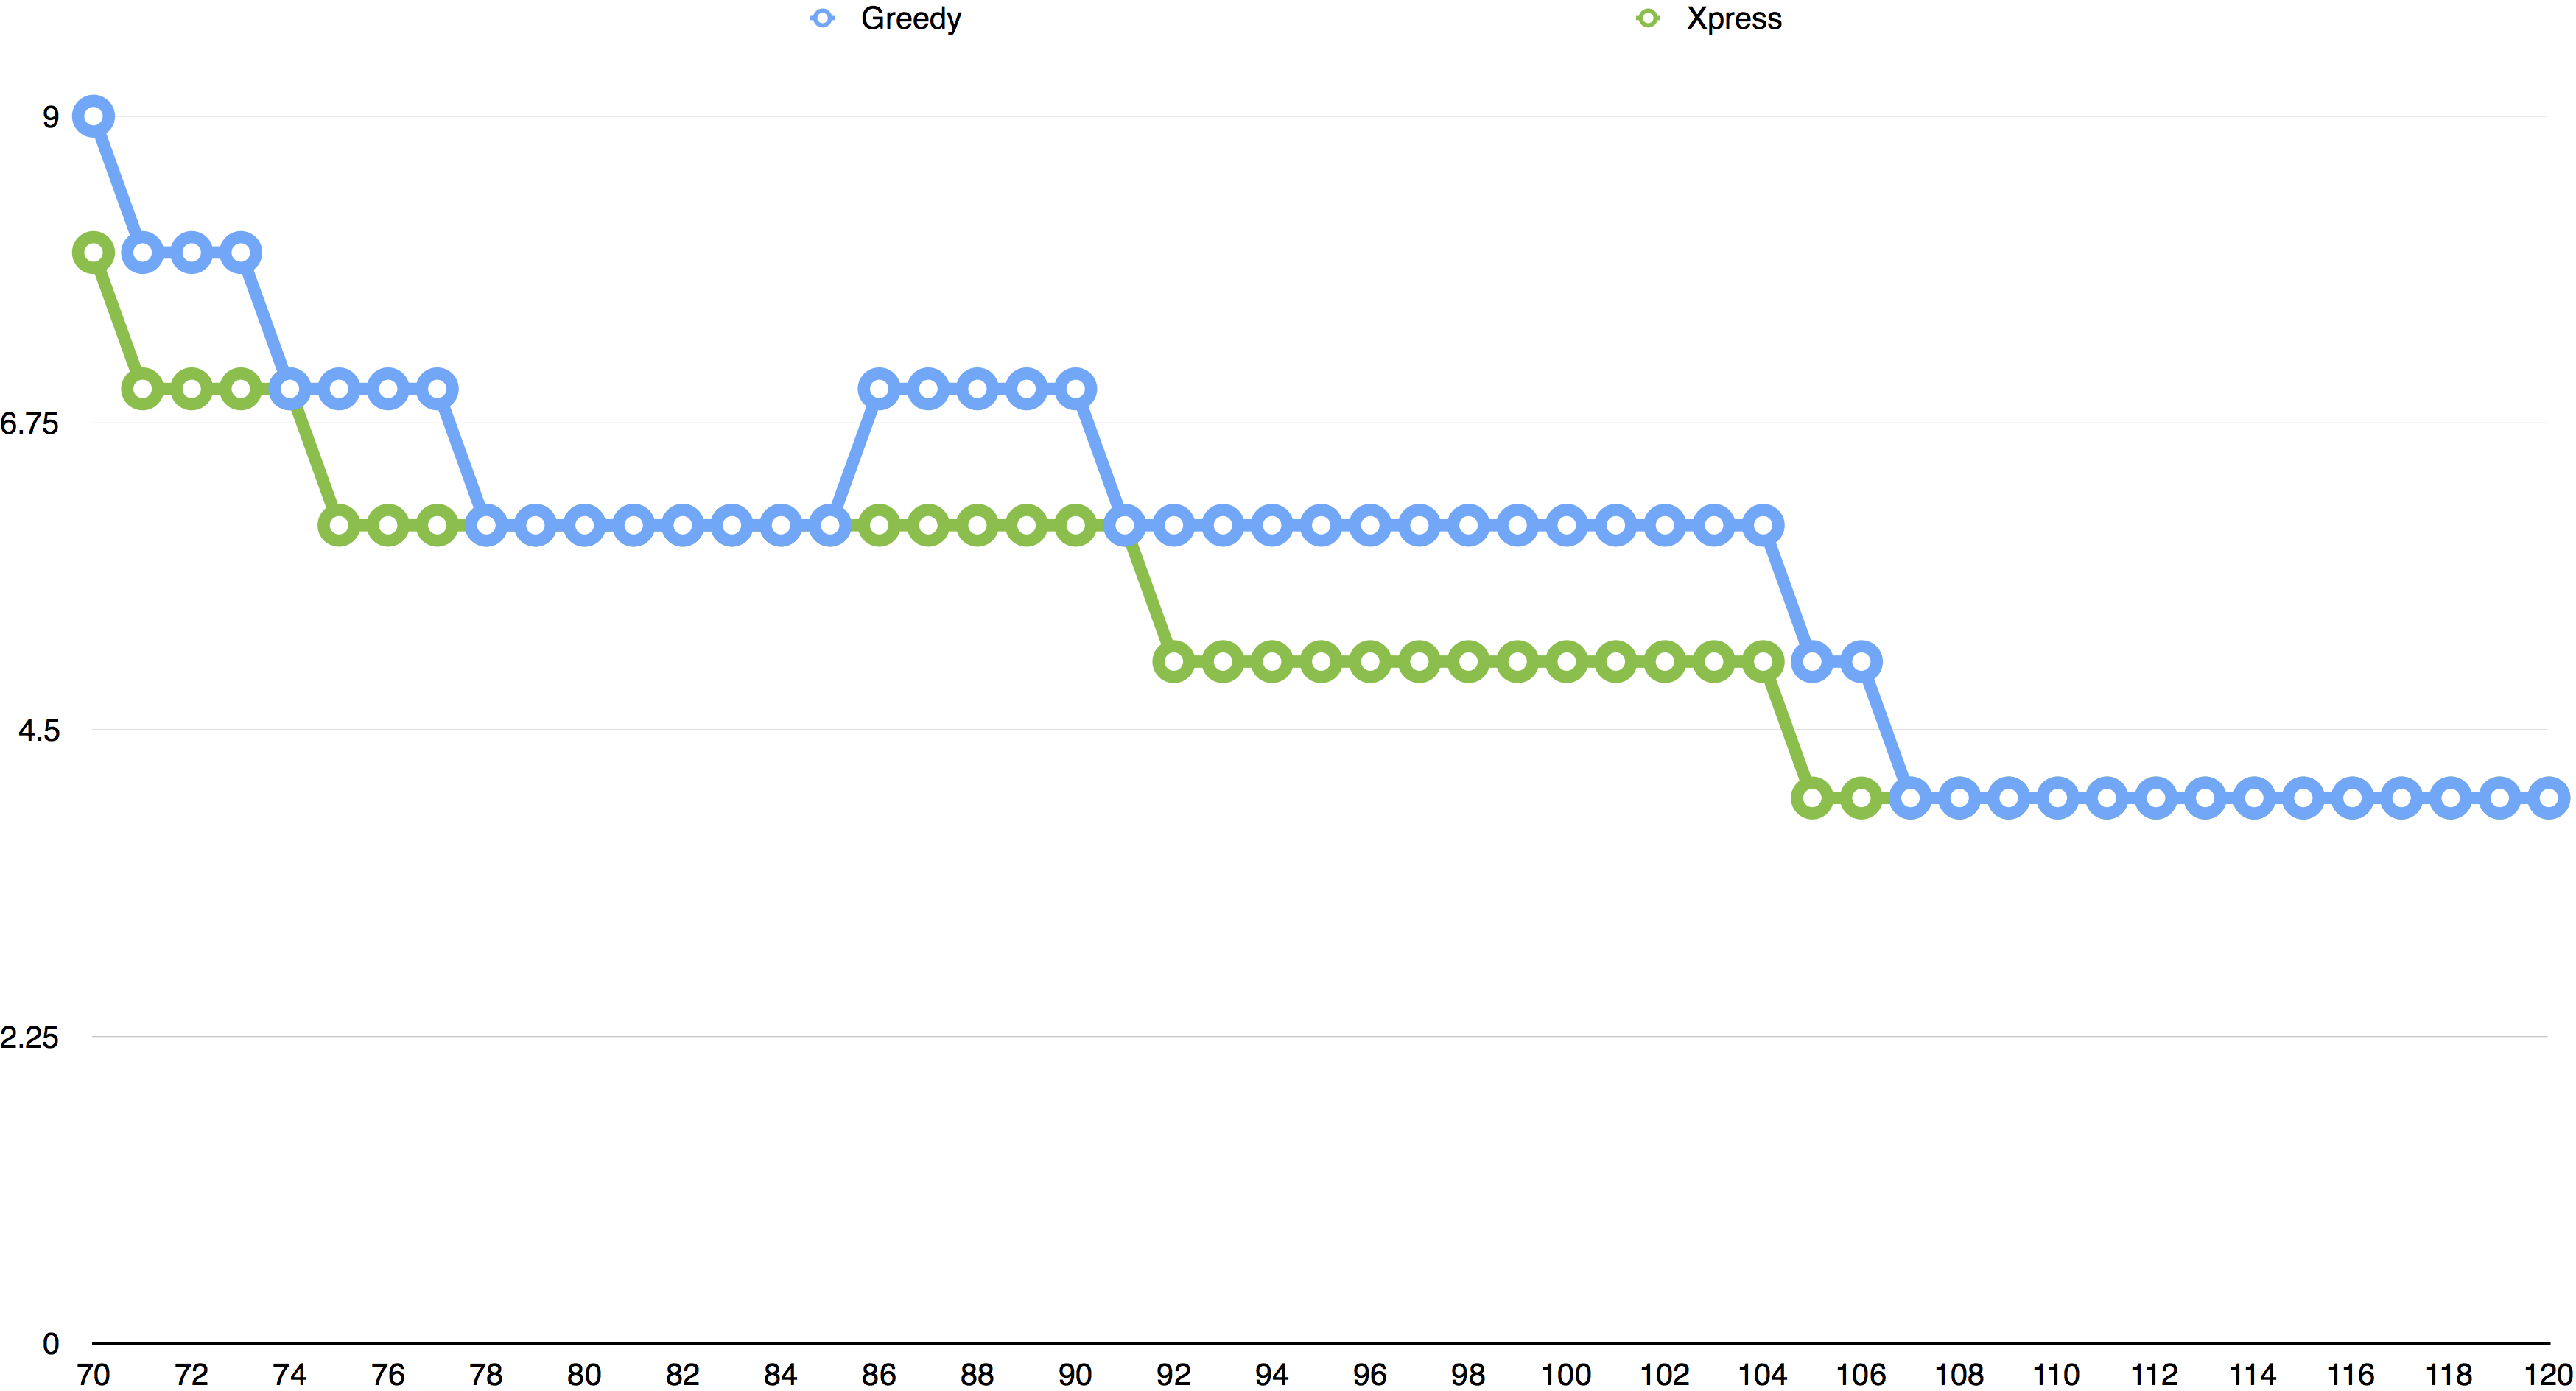
\includegraphics[width=0.8\textwidth]{tema-3-p6-1}
				\end{center}
				\caption{[TODO ]}
				\label{}
			\end{figure}


			\begin{table}[h]
				\begin{center}
					\csvautotabular{../results/csv/tema-3-p6-1.csv}
				\end{center}
				\caption{[TODO ]}
				\label{}
			\end{table}

		\subsection{Ejercicio \emph{aint1}}
		\label{sec:e-6.2a}

			\paragraph{}
			[TODO ]


			\begin{figure}[h]
				\begin{center}
					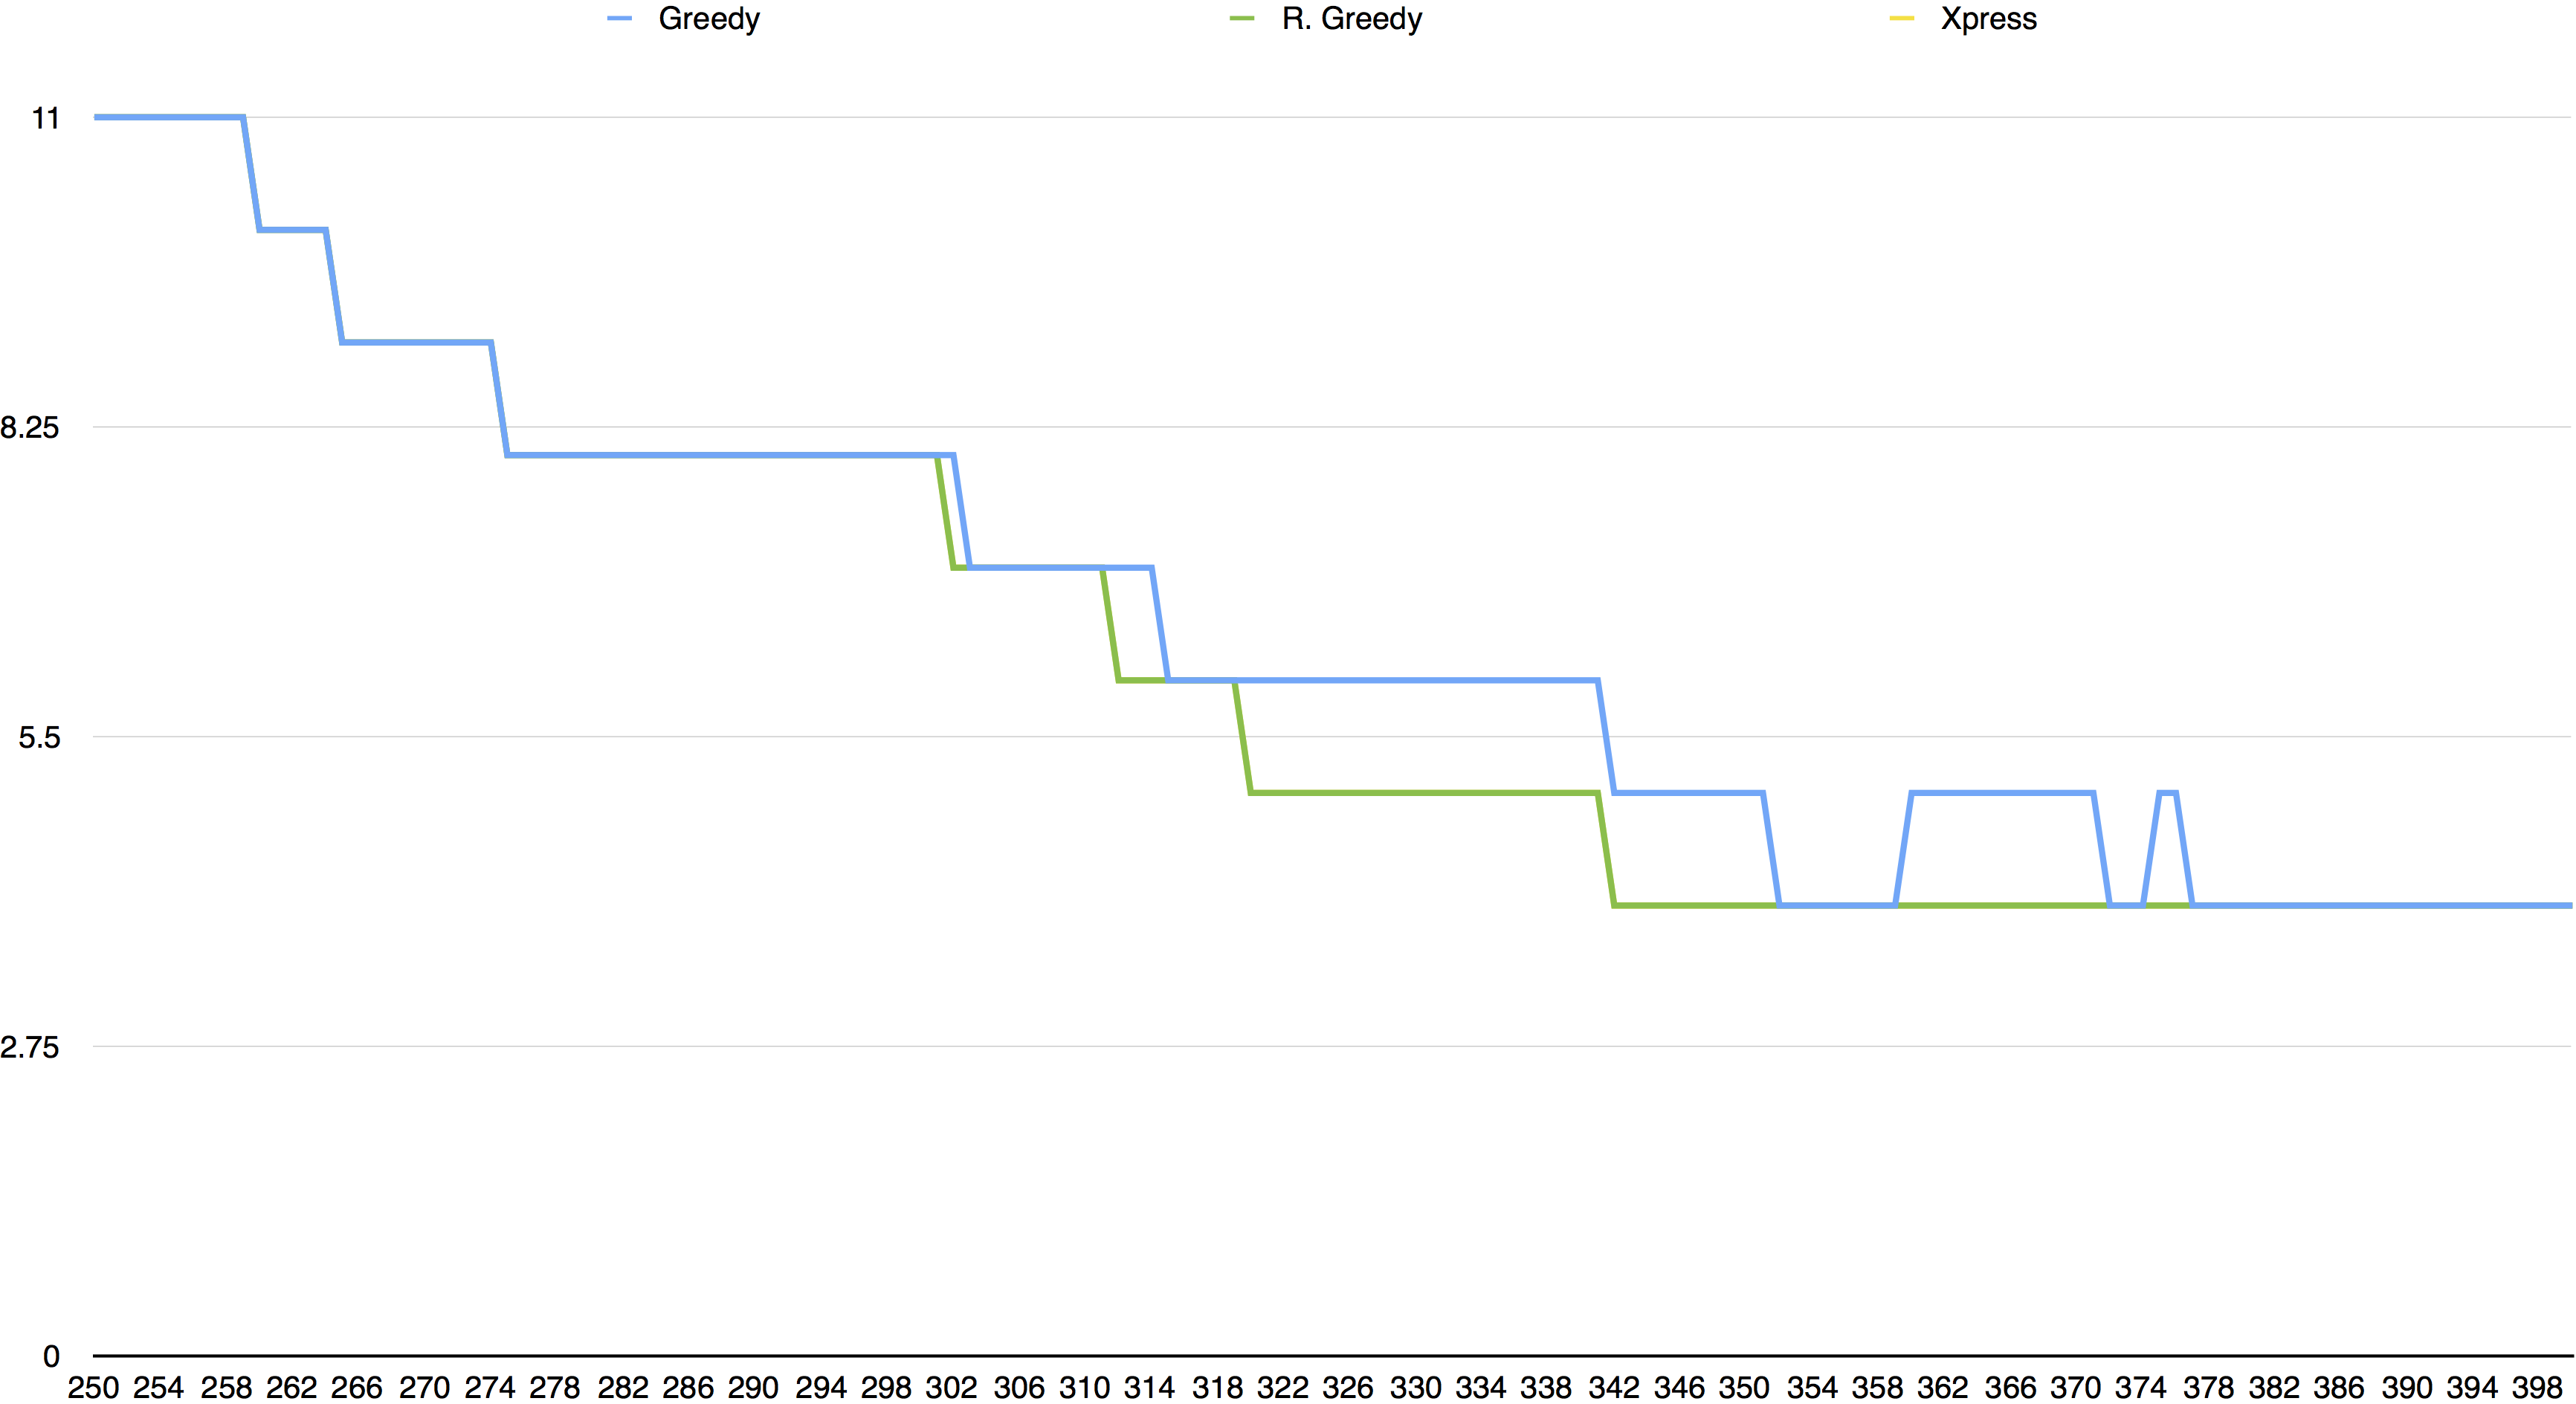
\includegraphics[width=0.8\textwidth]{tema-3-p6-2-a}
				\end{center}
				\caption{[TODO ]}
				\label{}
			\end{figure}

			\begin{table}[h]
				\begin{center}
					\csvautotabular{../results/csv/tema-3-p6-2-a-1.csv}
				\end{center}
				\caption{[TODO ]}
				\label{}
			\end{table}

			\begin{table}[h]
				\begin{center}
					\csvautotabular{../results/csv/tema-3-p6-2-a-2.csv}
				\end{center}
				\caption{[TODO ]}
				\label{}
			\end{table}

			\begin{table}[h]
				\begin{center}
					\csvautotabular{../results/csv/tema-3-p6-2-a-3.csv}
				\end{center}
				\caption{[TODO ]}
				\label{}
			\end{table}

		\subsection{Ejercicio \emph{aint5}}
		\label{sec:e-6.2b}

			\paragraph{}
			[TODO ]

			\begin{figure}[h]
				\begin{center}
					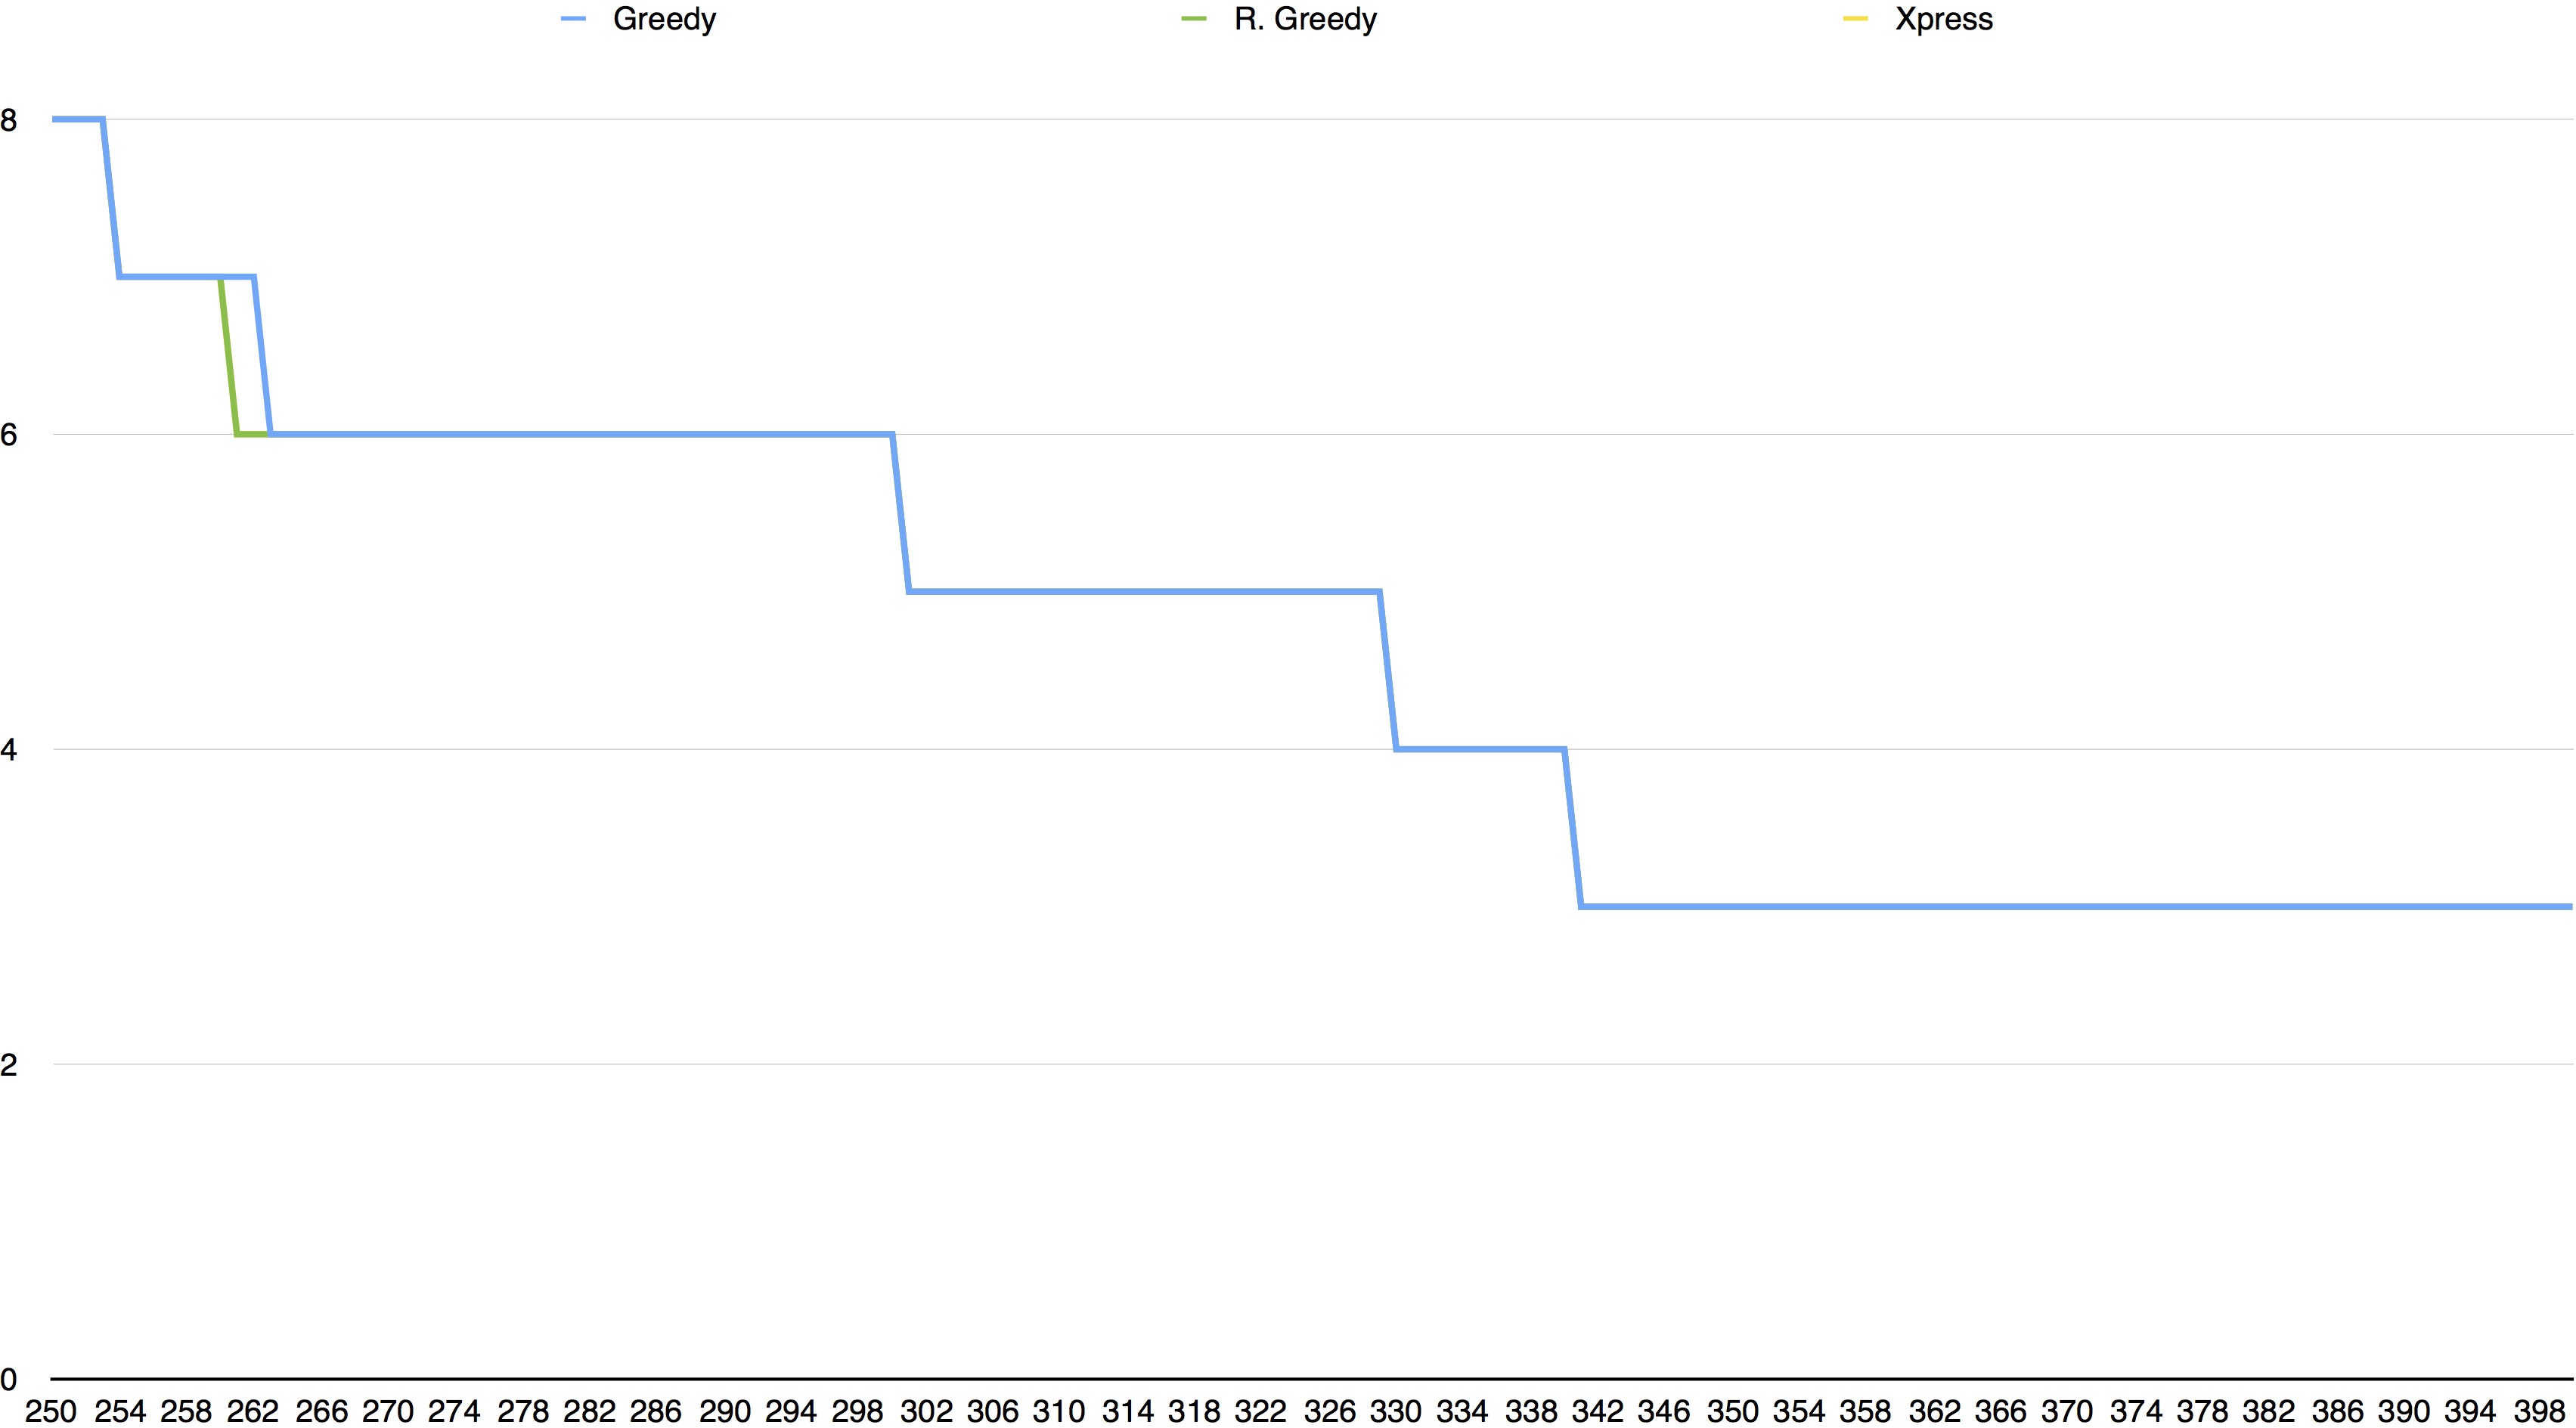
\includegraphics[width=0.8\textwidth]{tema-3-p6-2-b}
				\end{center}
				\caption{[TODO ]}
				\label{}
			\end{figure}

			\begin{table}[h]
				\begin{center}
					\csvautotabular{../results/csv/tema-3-p6-2-b-1.csv}
				\end{center}
				\caption{[TODO ]}
				\label{}
			\end{table}

			\begin{table}[h]
				\begin{center}
					\csvautotabular{../results/csv/tema-3-p6-2-b-2.csv}
				\end{center}
				\caption{[TODO ]}
				\label{}
			\end{table}

			\begin{table}[h]
				\begin{center}
					\csvautotabular{../results/csv/tema-3-p6-2-b-3.csv}
				\end{center}
				\caption{[TODO ]}
				\label{}
			\end{table}

	\section{Max-Covering Problem}
	\label{sec:e-7}

		\paragraph{}
		[TODO ]

		\begin{eqfloat}
			\begin{equation}
				\begin{array}{ll@{}ll}
					\text{Maximizar}
						& \displaystyle\sum\limits_{i = 1}^{m} h_{i} & z_{i} 			&							\\
					\text{sujeto a}
						& \displaystyle\sum\limits_{j \in N_i}& x_{j} \geq z_i,		&i=1 ,..., m	\\
						& \displaystyle\sum\limits_{j = 1}^n 	& x_{j} \leq p,  		& 						\\
						&                                     &	x_{j} \in \{0,1\},&j=1 ,..., n 	\\
						&                                     &	z_{i} \in \{0,1\},&i=1 ,..., m  \\
				\end{array}
			\end{equation}
			\caption{Formulación de \emph{Max-Covering Problem}.}
			\label{eq:max_covering}
		\end{eqfloat}


		\subsection{Ejercicio \emph{aint1}}
		\label{sec:e-7a}

			\paragraph{}
			[TODO ]

			\begin{figure}[h]
				\begin{center}
					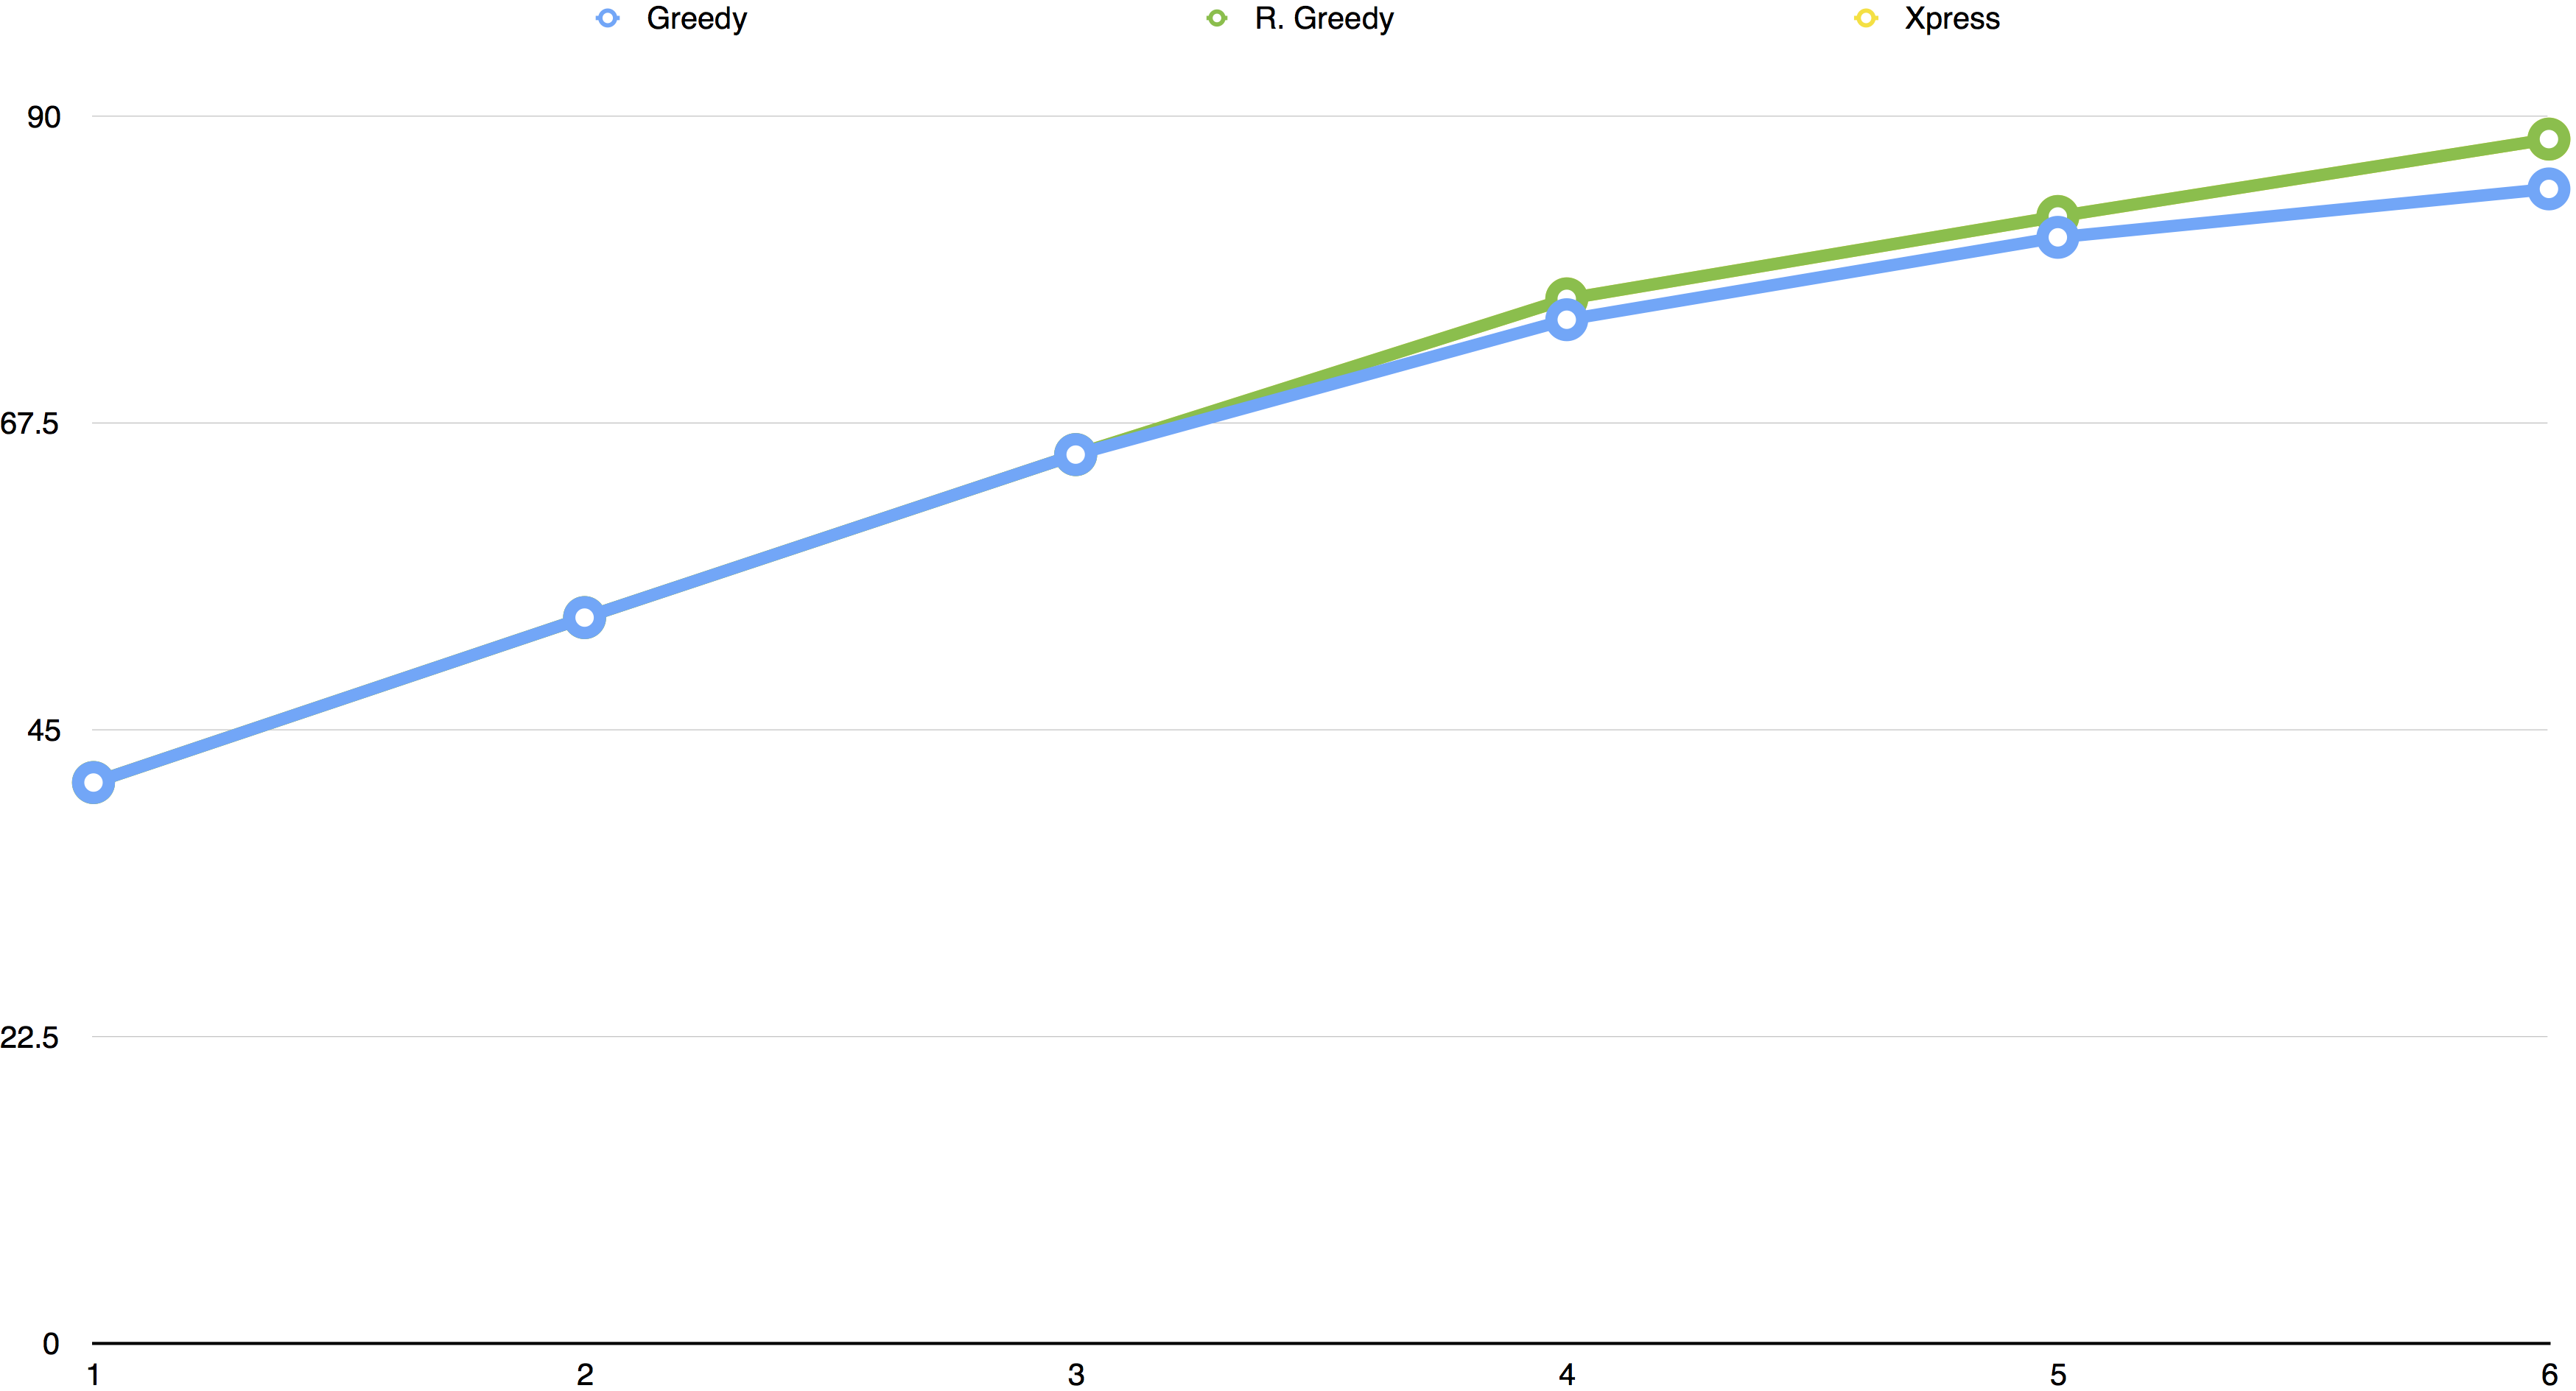
\includegraphics[width=0.8\textwidth]{tema-3-p7-a}
				\end{center}
				\caption{[TODO ]}
				\label{}
			\end{figure}

			\begin{table}[h]
				\begin{center}
					\csvautotabular{../results/csv/tema-3-p7-a.csv}
				\end{center}
				\caption{[TODO ]}
				\label{}
			\end{table}

		\subsection{Ejercicio \emph{aint5}}
		\label{sec:e-7b}

			\paragraph{}
			[TODO ]

			\begin{figure}[h]
				\begin{center}
					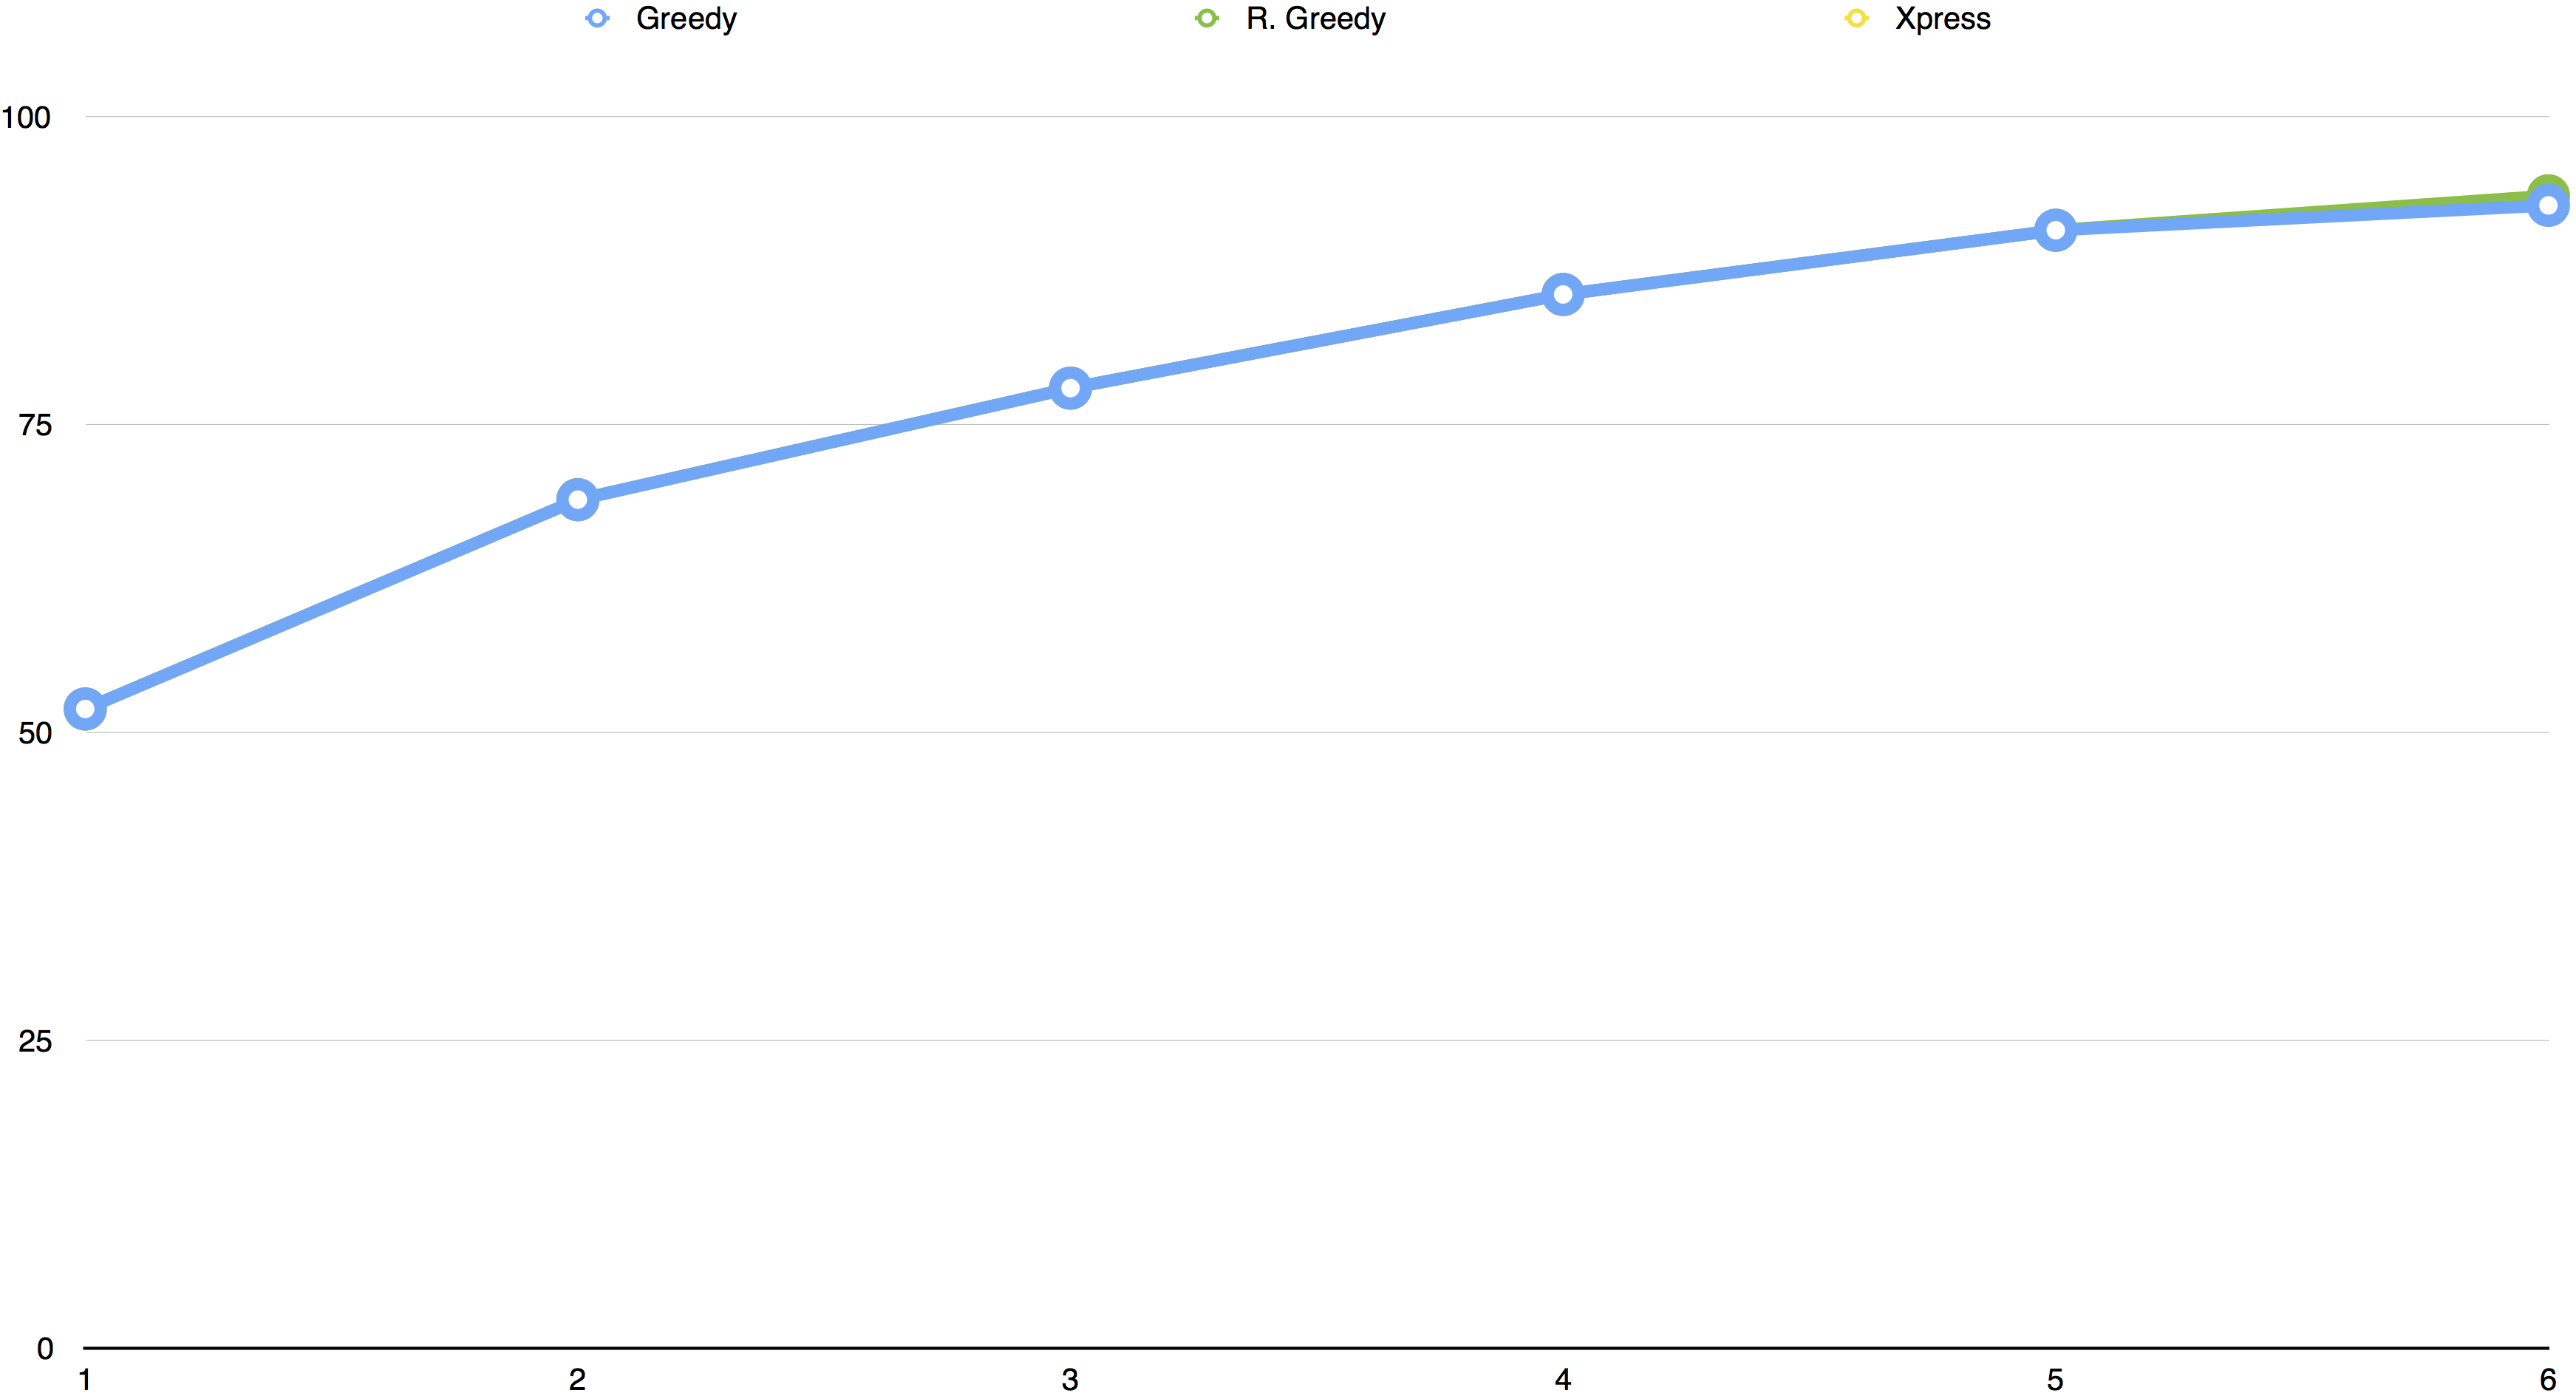
\includegraphics[width=0.8\textwidth]{tema-3-p7-b}
				\end{center}
				\caption{[TODO ]}
				\label{}
			\end{figure}

			\begin{table}[h]
				\begin{center}
					\csvautotabular{../results/csv/tema-3-p7-b.csv}
				\end{center}
				\caption{[TODO ]}
				\label{}
			\end{table}


	\section{P-Median Problem}
	\label{sec:e-8}

		\paragraph{}
		[TODO ]


		\begin{eqfloat}
			\begin{equation}
				\begin{array}{ll@{}ll}
					\text{Minimizar}
						& \displaystyle\sum\limits_{i = 1}^m
							\displaystyle\sum\limits_{j = 1}^n	& h_i d_{ij} y_{ij}	&							\\
					\text{sujeto a}
						& \displaystyle\sum\limits_{j = 1}^n 	& y_{ij} = 1,		& i = 1,..., m	\\
						& 																	 	& y_{ij} \leq x_{j},  		& i=1 ,..., m,j=1 ,..., n  \\
						& \displaystyle\sum\limits_{j = 1}^n 	& x_{j} = p,  		& 						\\
						&                                     &	x_{j} \in \{0,1\},&j=1 ,..., n 	\\
						&                                     &	y_{ij} \in \{0,1\},&i=1 ,..., m, j=1 ,..., n  \\
				\end{array}
			\end{equation}
			\caption{Formulación de \emph{P-Median Problem}.}
      \label{eq:p_median}
    \end{eqfloat}


		\subsection{Ejercicio \emph{coordenadas\_15}}
		\label{sec:e-8a}

			\paragraph{}
			[TODO ]

			\begin{figure}[h]
				\begin{center}
					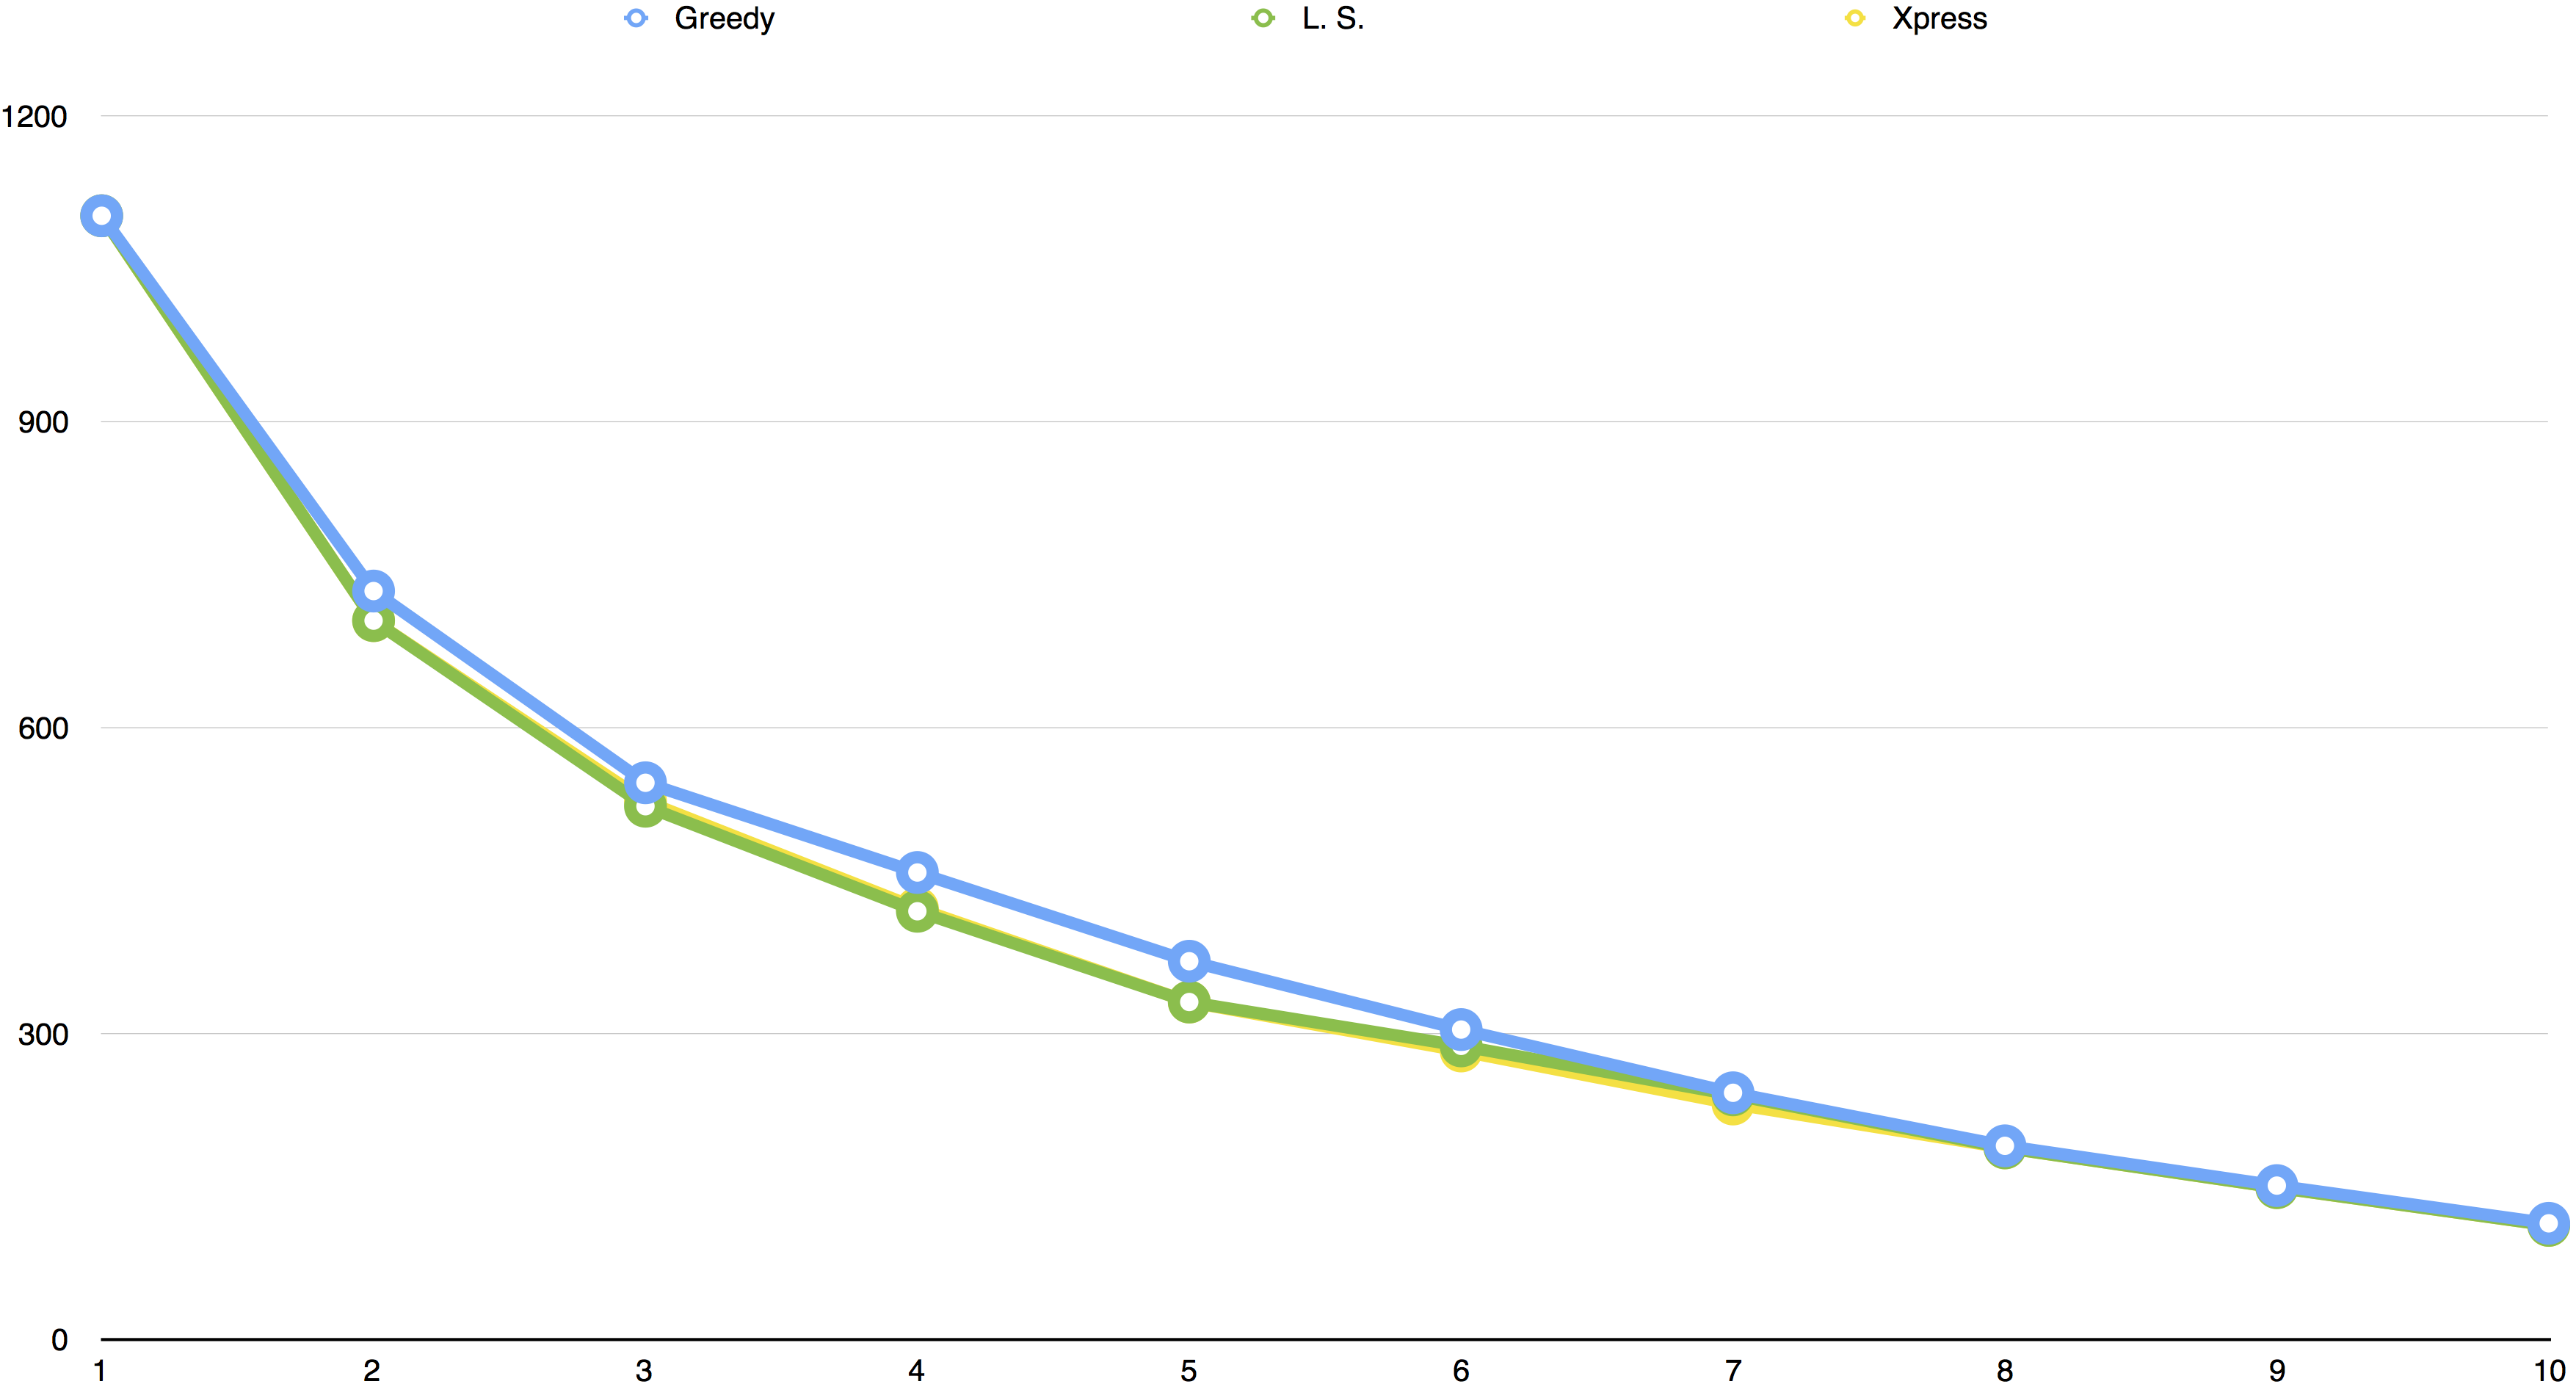
\includegraphics[width=0.8\textwidth]{tema-3-p8-a}
				\end{center}
				\caption{[TODO ]}
				\label{}
			\end{figure}

			\begin{figure}[h]
				\begin{center}
					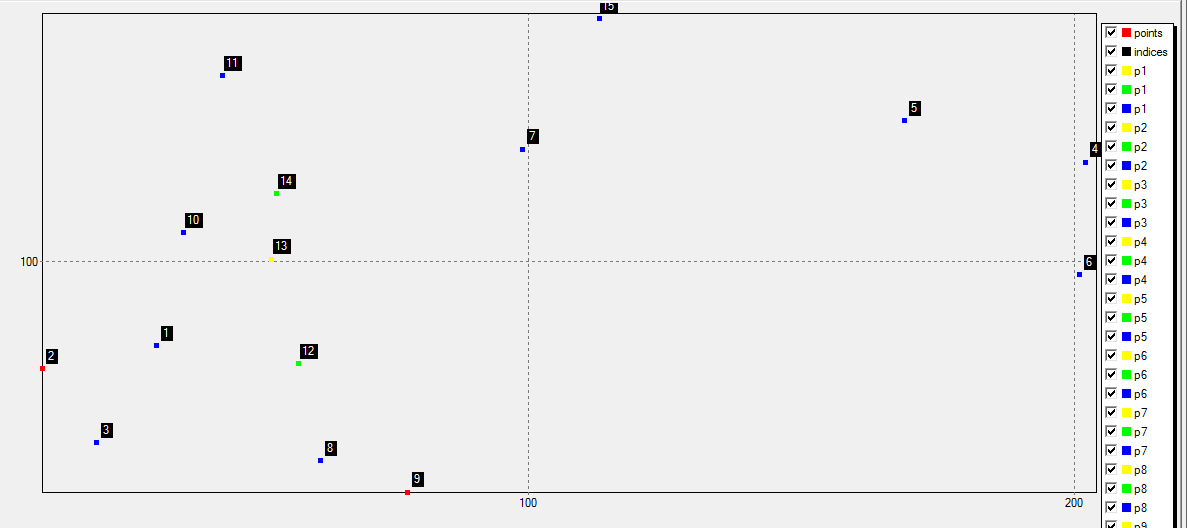
\includegraphics[width=0.8\textwidth]{tema-3-p8-a-graph}
				\end{center}
				\caption{[TODO ]}
				\label{}
			\end{figure}

			\begin{table}[h]
				\begin{center}
					\csvautotabular{../results/csv/tema-3-p8-a.csv}
				\end{center}
				\caption{[TODO ]}
				\label{}
			\end{table}


		\subsection{Ejercicio \emph{coordenadas\_30}}
		\label{sec:e-8b}

			\paragraph{}
			[TODO ]

			\begin{figure}[h]
				\begin{center}
					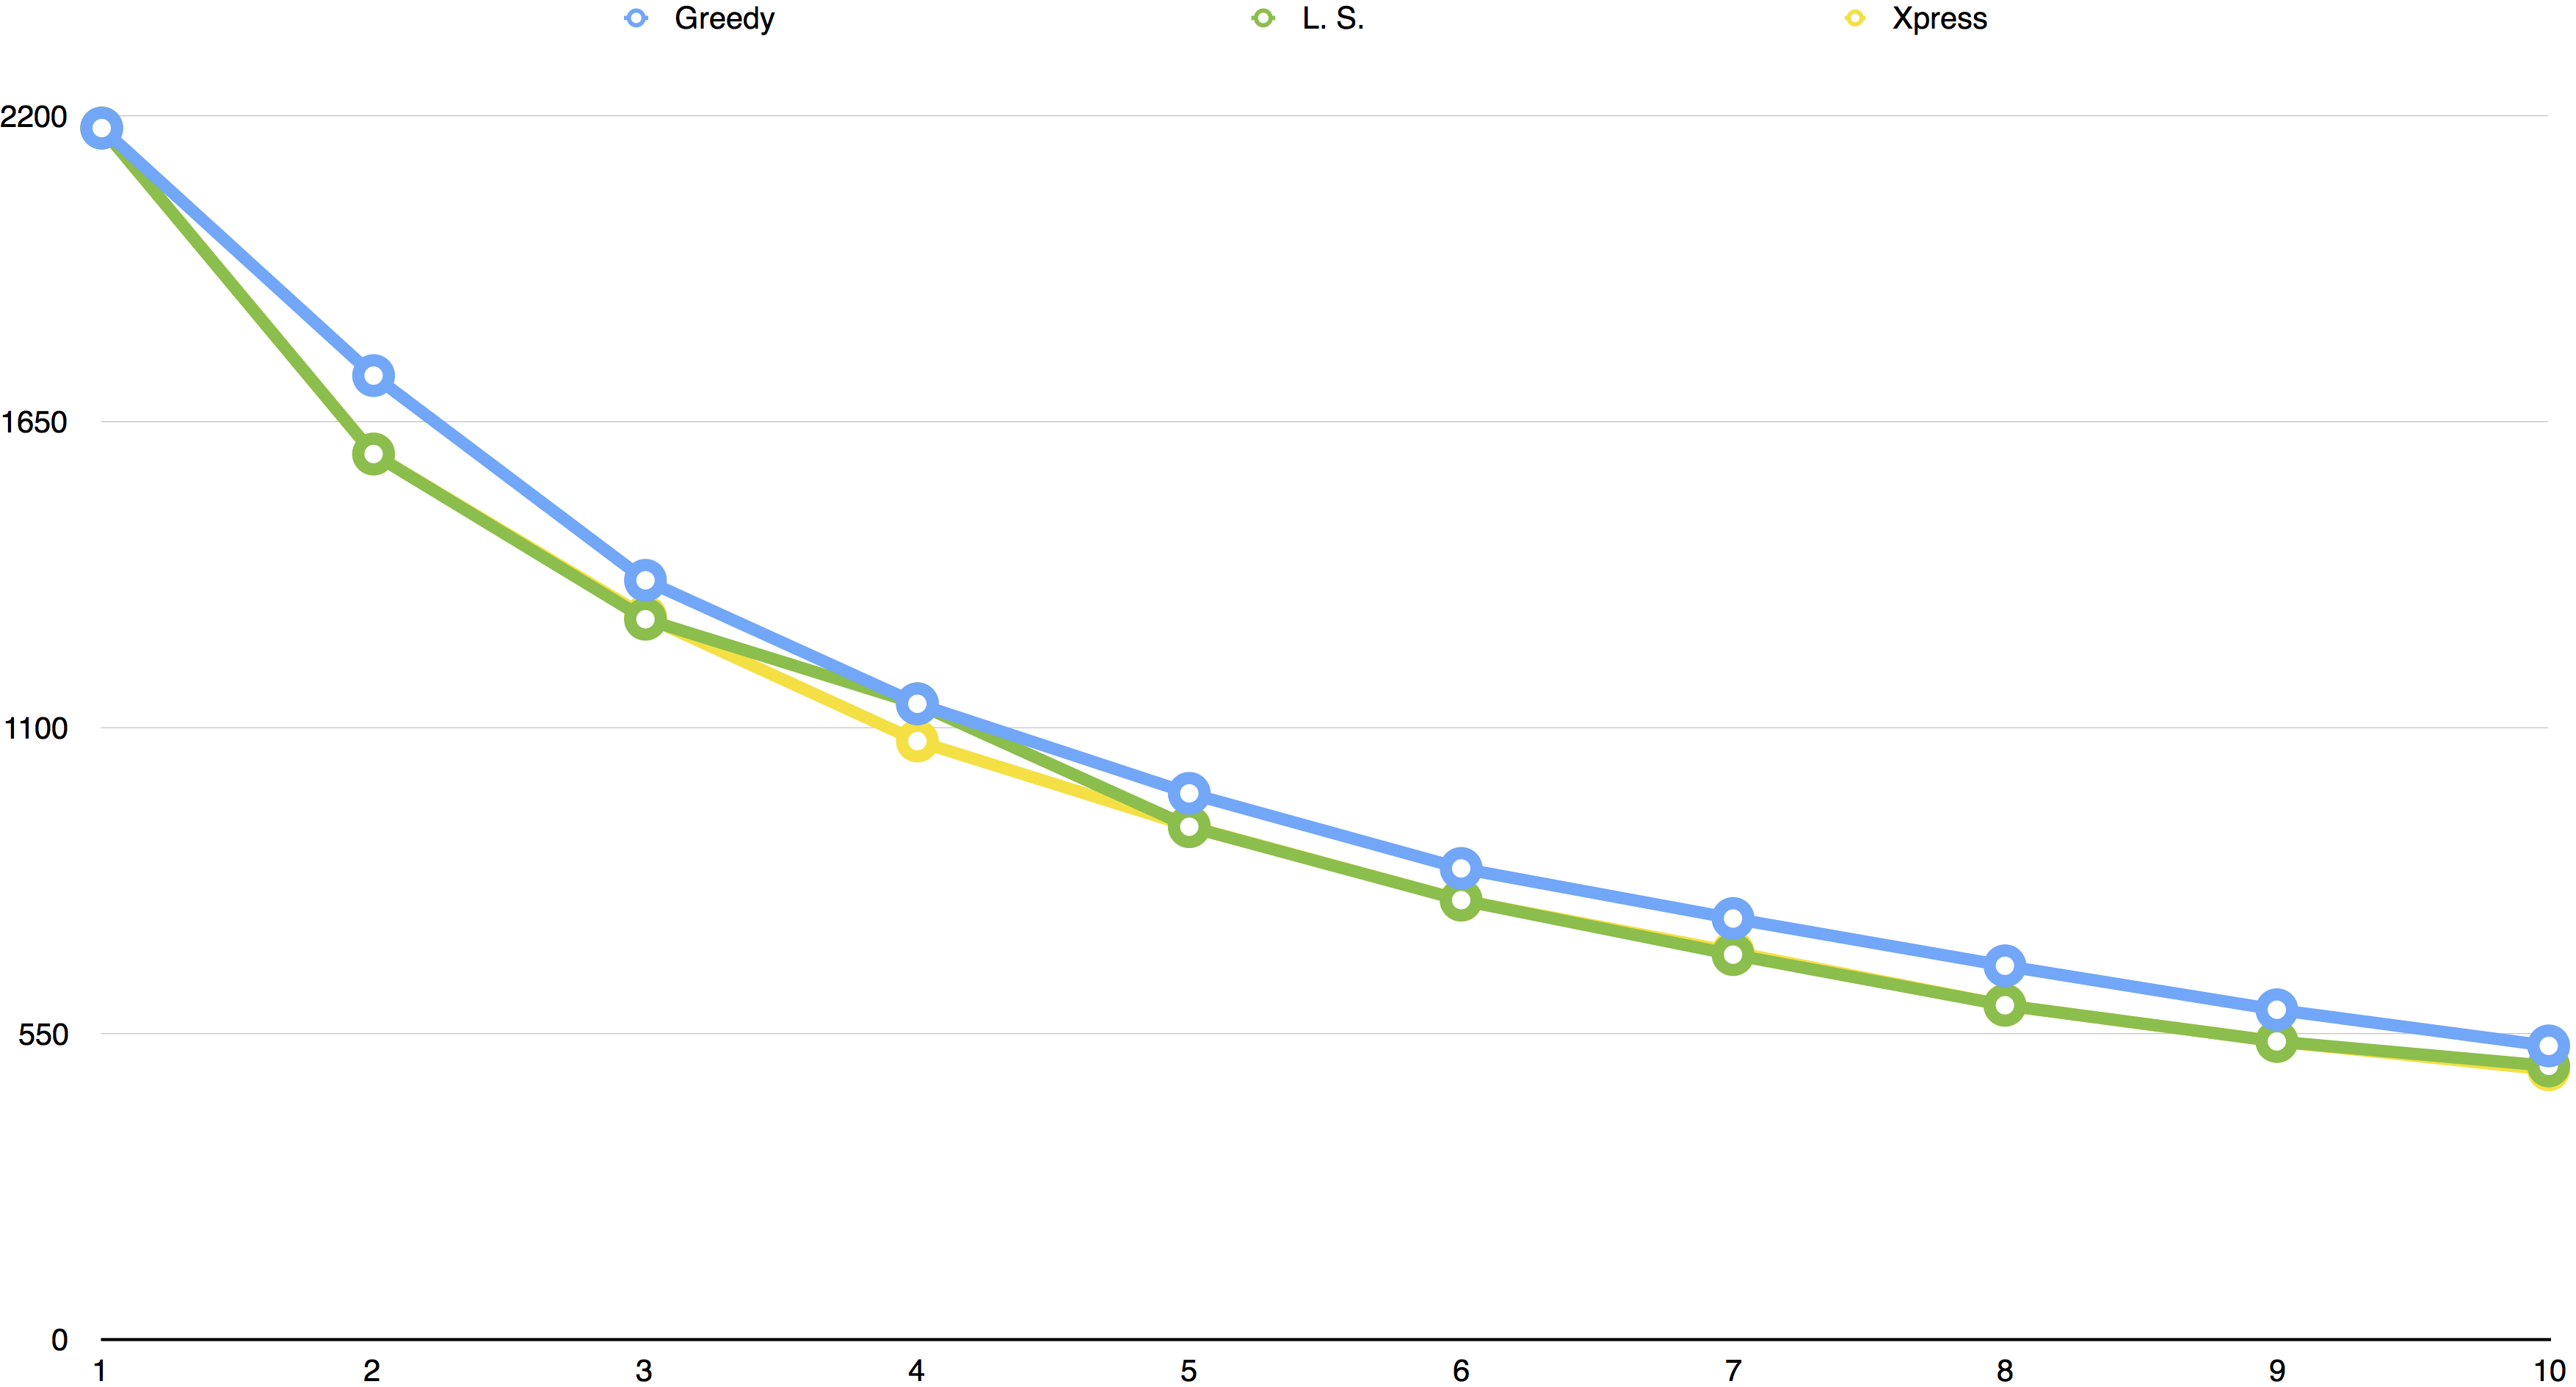
\includegraphics[width=0.8\textwidth]{tema-3-p8-b}
				\end{center}
				\caption{[TODO ]}
				\label{}
			\end{figure}

			\begin{figure}[h]
				\begin{center}
					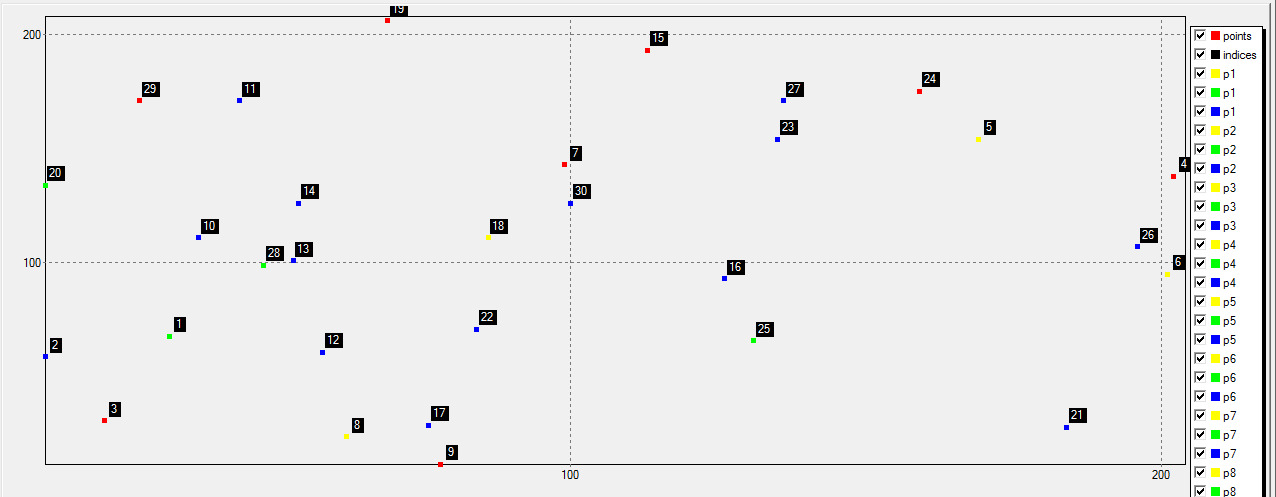
\includegraphics[width=0.8\textwidth]{tema-3-p8-b-graph}
				\end{center}
				\caption{[TODO ]}
				\label{}
			\end{figure}

			\begin{table}[h]
				\begin{center}
					\csvautotabular{../results/csv/tema-3-p8-b.csv}
				\end{center}
				\caption{[TODO ]}
				\label{}
			\end{table}

		\subsection{Ejercicio \emph{coordenadas\_100}}
		\label{sec:e-8c}

			\paragraph{}
			[TODO ]

			\begin{figure}[h]
				\begin{center}
					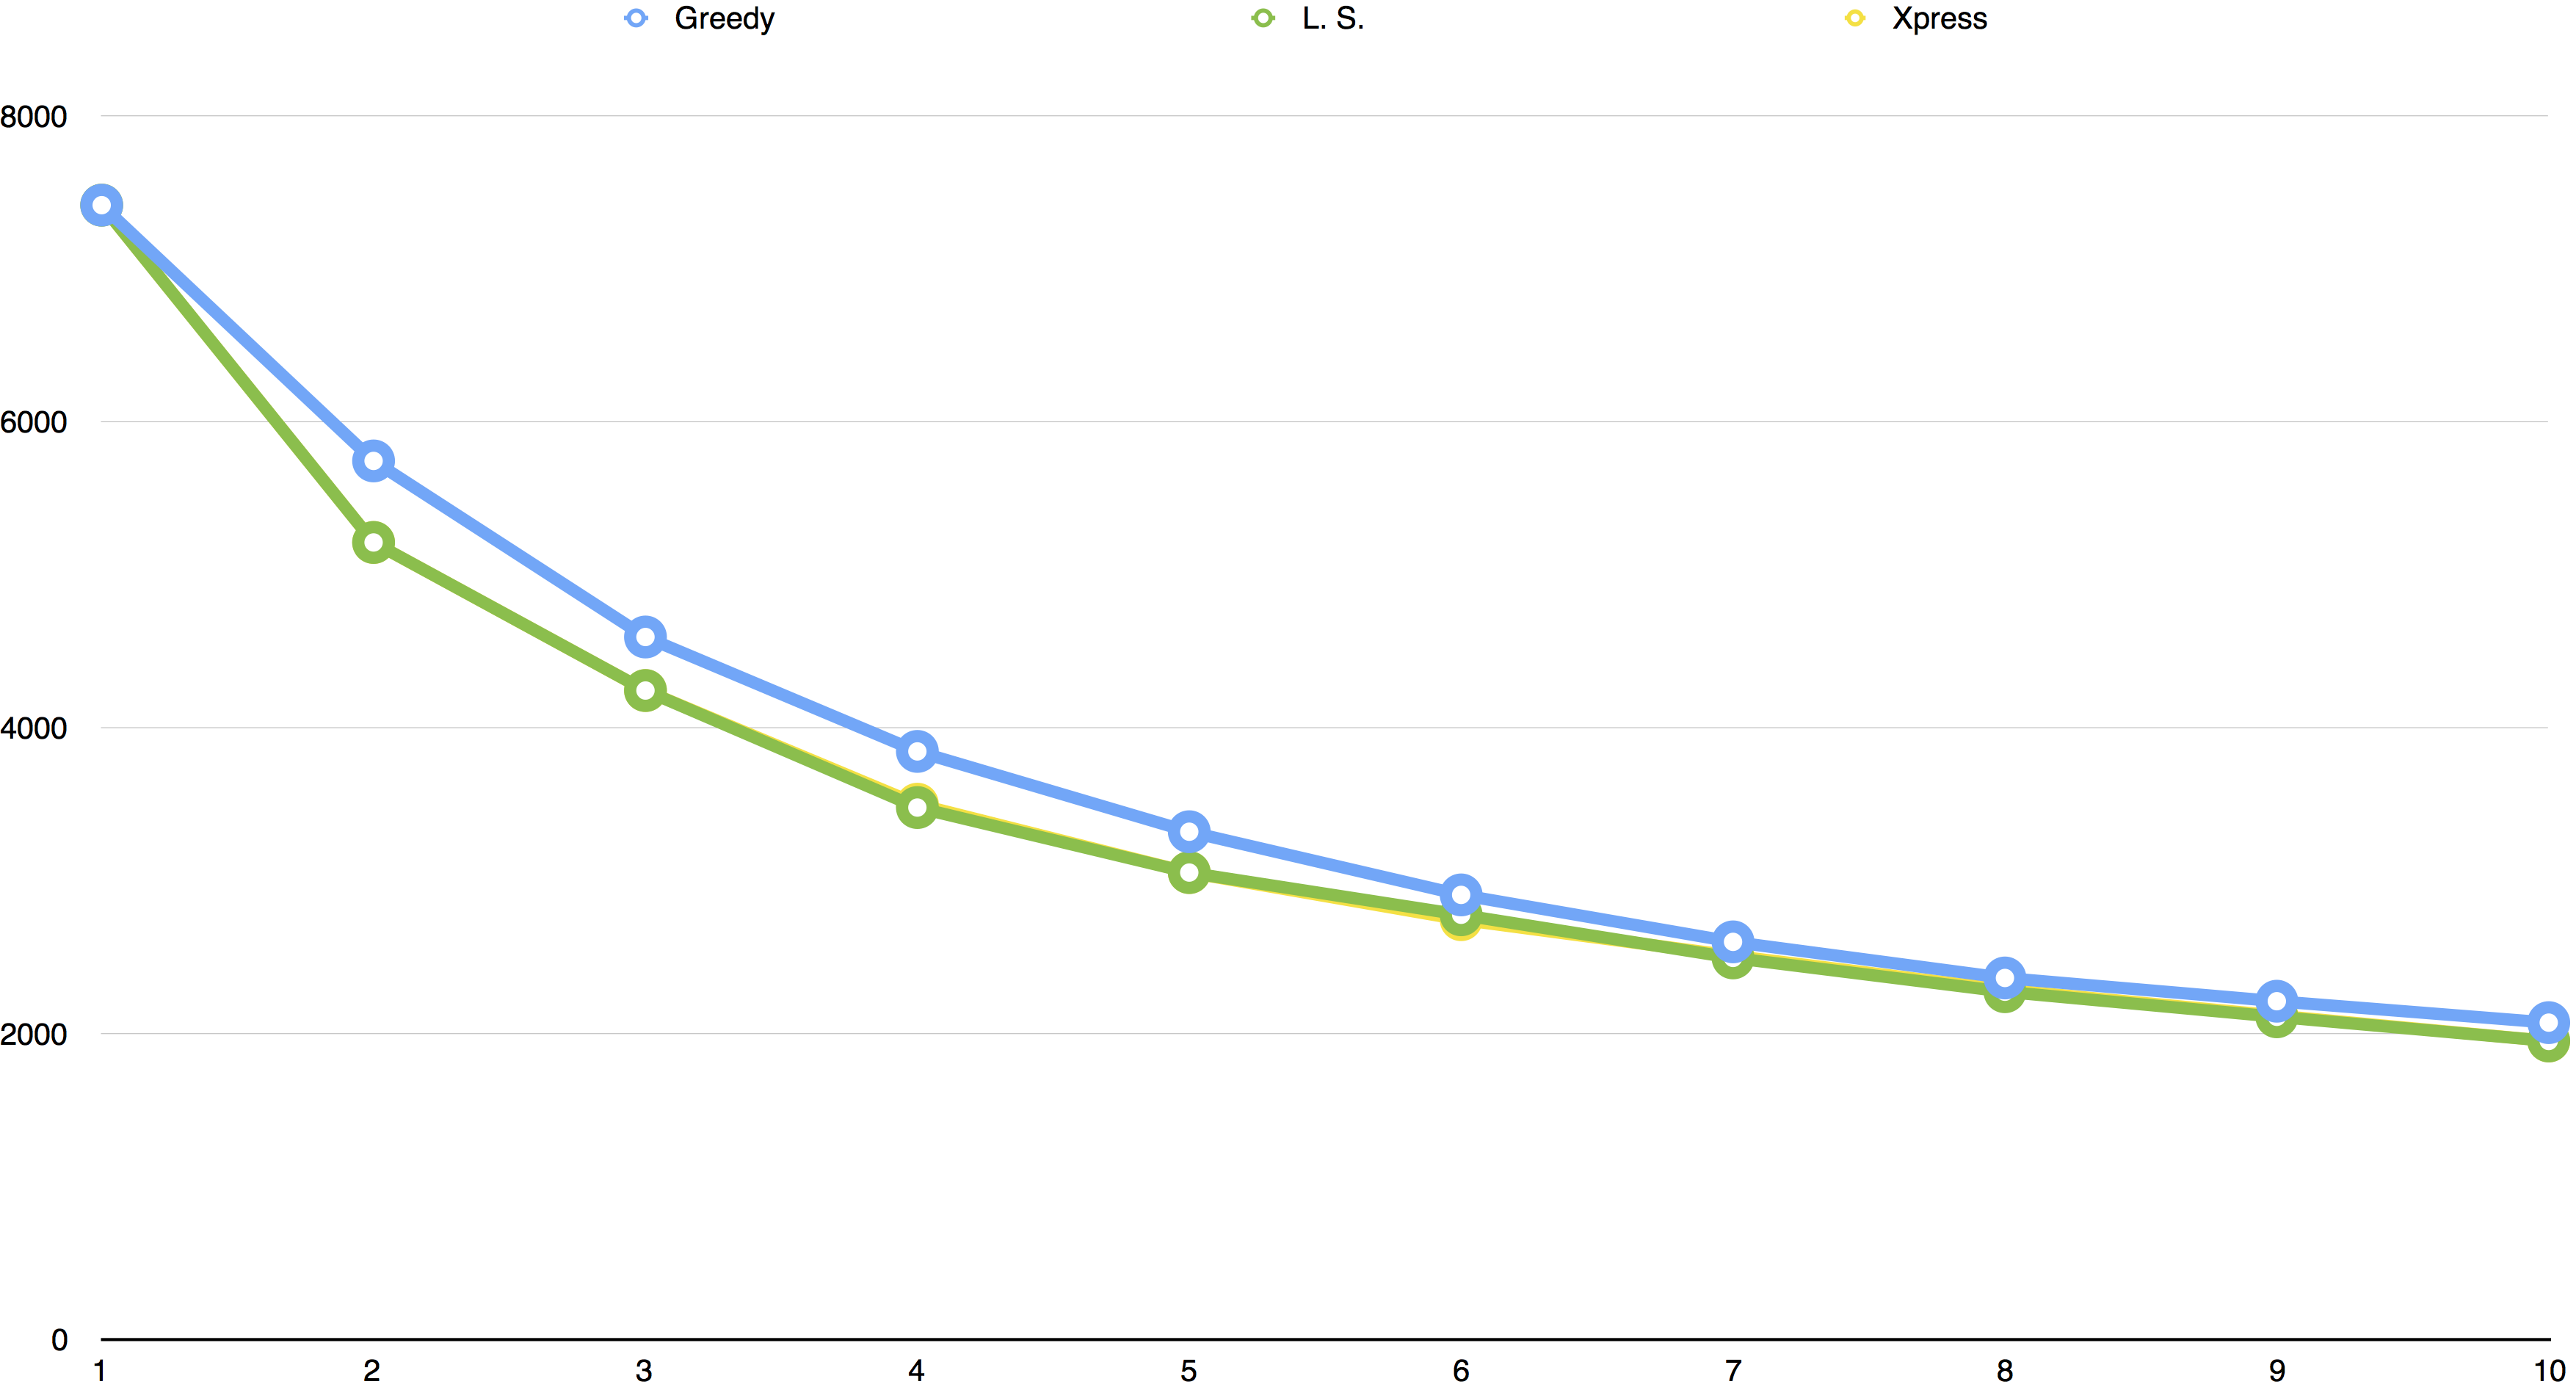
\includegraphics[width=0.8\textwidth]{tema-3-p8-c}
				\end{center}
				\caption{[TODO ]}
				\label{}
			\end{figure}

			\begin{figure}[h]
				\begin{center}
					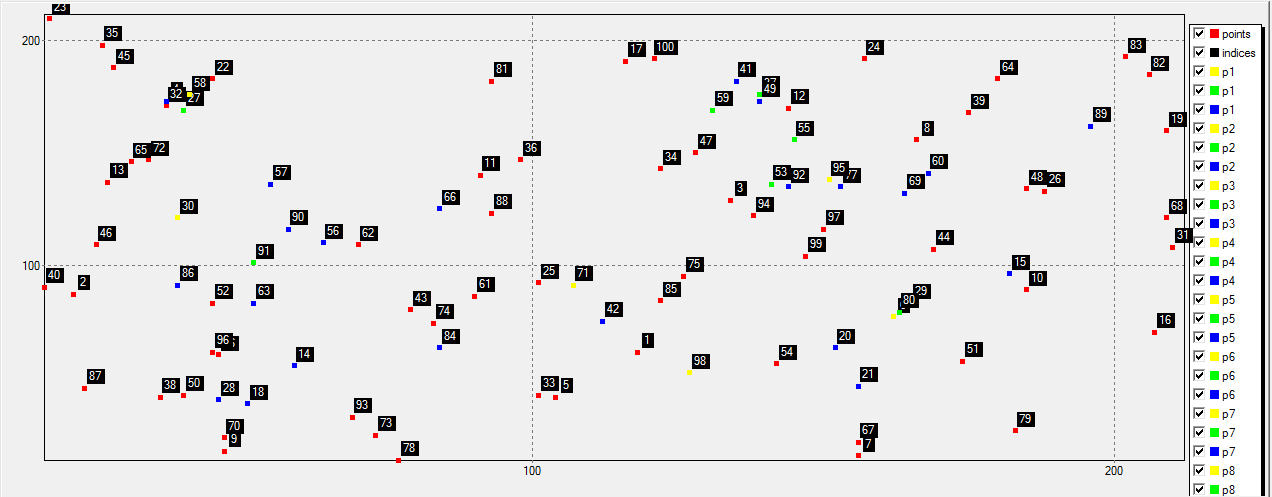
\includegraphics[width=0.8\textwidth]{tema-3-p8-c-graph}
				\end{center}
				\caption{[TODO ]}
				\label{}
			\end{figure}

			\begin{table}[h]
				\begin{center}
					\csvautotabular{../results/csv/tema-3-p8-c.csv}
				\end{center}
				\caption{[TODO ]}
				\label{}
			\end{table}

%-----------------------------
%	BIBLIOGRAPHY
%-----------------------------
	\nocite{subject:mio}
	\nocite{garciparedes:mosel-examples}
	\bibliographystyle{acm}
  \bibliography{bib/misc}

\end{document}
